% !TEX program = pdflatex
\documentclass{article}
\usepackage{tikz}
\usetikzlibrary{matrix,arrows.meta}

\begin{document}
\section*{Neighbouring rack cells}
\begin{figure}[ht]\centering
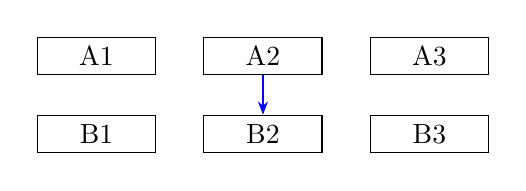
\begin{tikzpicture}

\matrix (m) [matrix of nodes,nodes={draw,minimum width=15mm},row sep=5mm,column sep=6mm]{
 A1 & A2 & A3 \\ B1 & B2 & B3 \\};
\draw[-{Stealth},blue] (m-1-2)--(m-2-2);
\end{tikzpicture}\caption{Move down one row while keeping the column fixed.}\end{figure}
\end{document}
